\documentclass[
	tikz,
	border=3pt,
]{standalone}


\usepackage{cbc_frames_tikz}



\begin{document}
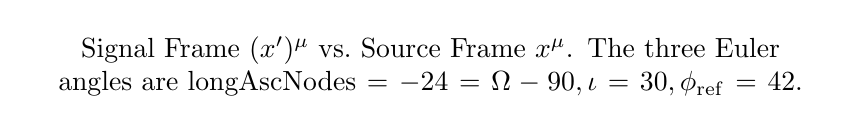
\begin{tikzpicture}
	\drawframes[%
		inclination=30,
		longascnodes=-24,
		phiref=42,
		eccentricity=0.5,
		showcelestialframe=false,
		axislabelpad=0.16,
	];
	
	\node[text width=10cm, align=center] at (-4, -6) {Signal Frame $(x')^\mu$ vs.~Source Frame $x^\mu$. The three Euler angles are $\mathrm{longAscNodes} = -24 = \Omega - 90, \iota = 30, \phi_\mathrm{ref} = 42$.};
\end{tikzpicture}
\end{document}
